\documentclass[11pt]{article}

\usepackage[letterpaper,margin=0.75in]{geometry}
\usepackage{booktabs}
\usepackage{caption}
\usepackage{graphicx}
\usepackage{listings}
\usepackage{float}
\usepackage{scrextend}
\usepackage{hyperref}
\usepackage[parfill]{parskip}
\renewcommand{\lstlistingname}{Snippet}


\begin{document}

\lstset{
  language=Python,
  basicstyle=\small,          % print whole listing small
  keywordstyle=\bfseries,
  identifierstyle=,           % nothing happens
  commentstyle=,              % white comments
  stringstyle=\ttfamily,      % typewriter type for strings
  showstringspaces=false,     % no special string spaces
  numbers=left,
  numberstyle=\tiny,
  numbersep=5pt,
  frame=tb
}

\title{Congestion Control Part 2}

\author{Brandt Elison & Joe Eklund}

\date{March 31, 2016}

\maketitle

\section{Introduction}

The purpose of our project was to verify our implementation of TCP congestion control by testing using a series of experiments. We divided our experiments into two categories: basic and advanced. The basic experiments tested the performance of our implementation of TCP congestion control by varying the number of flows that concurrently transfer a 1 MB file over a single link between two hosts. The advanced experiments also manipulated the link congestion, but they altered the network topology and the way TCP responded to loss events.

\section{Basic Experiments}

For our basic experiments we created a two host network with the following parameters:

\begin{itemize}
  \item 10 ms - propagation delay
  \item 100 packets - queue size
  \item 10 Mbps - transmission rate
  \item 500,000 bytes - intitial slow start threshold
\end{itemize}

Each of the experiments uses a different number of flows, meaning a different number of connections transfering 1 MB files simultaneously on the link.

\subsection{One Flow}
  
\begin{figure}[H]
\caption{The graph of our one flow receiver's rate over time.}
	\label{figure1}
  	\centering
  	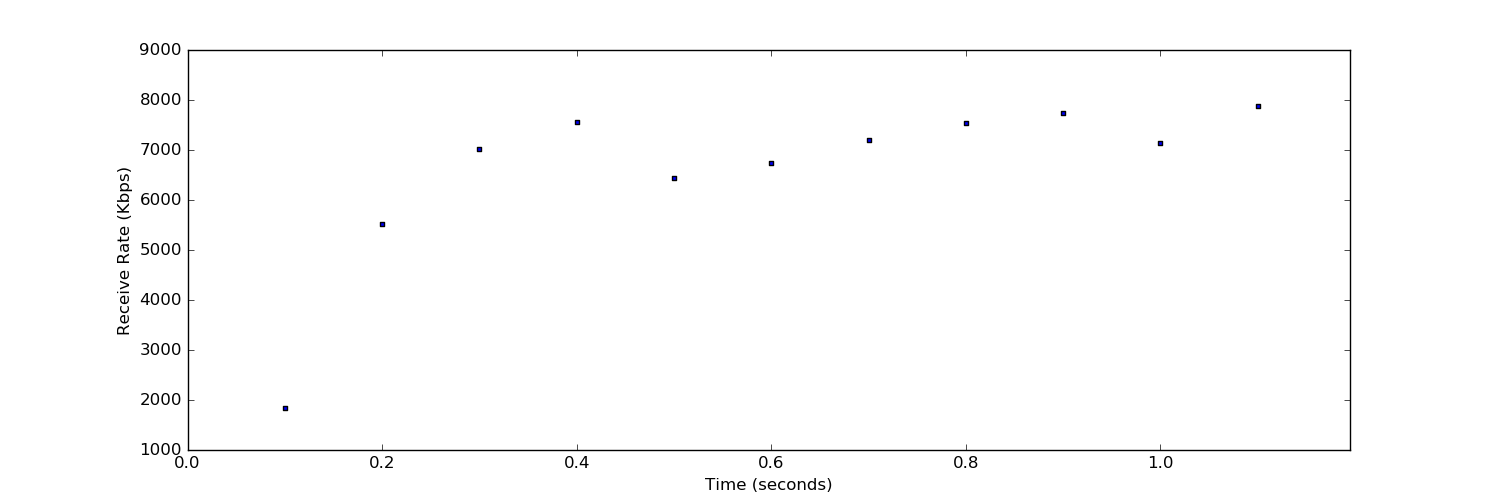
\includegraphics[width=\linewidth]{1f_rate.png}
\end{figure}

\begin{figure}[H]
\caption{The graph of our one flow queue size over time.}
  \label{figure2}
    \centering
    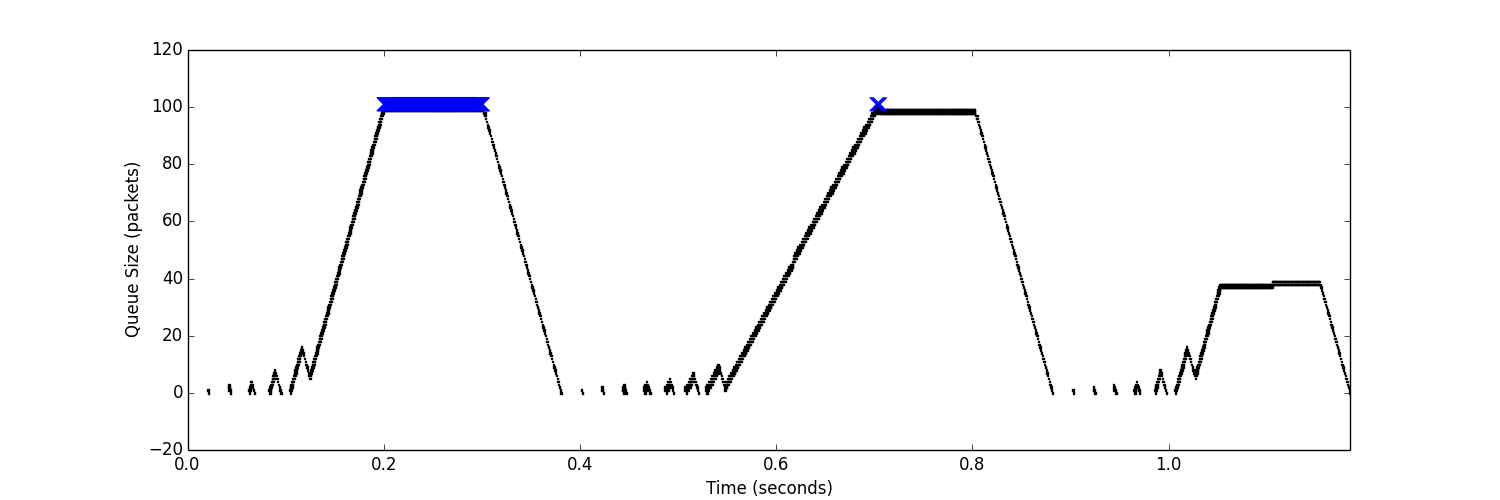
\includegraphics[width=\linewidth]{1f_queue.png}
\end{figure}

\begin{figure}[H]
\caption{The graph of our one flow congestion window size over time.}
  \label{figure3}
    \centering
    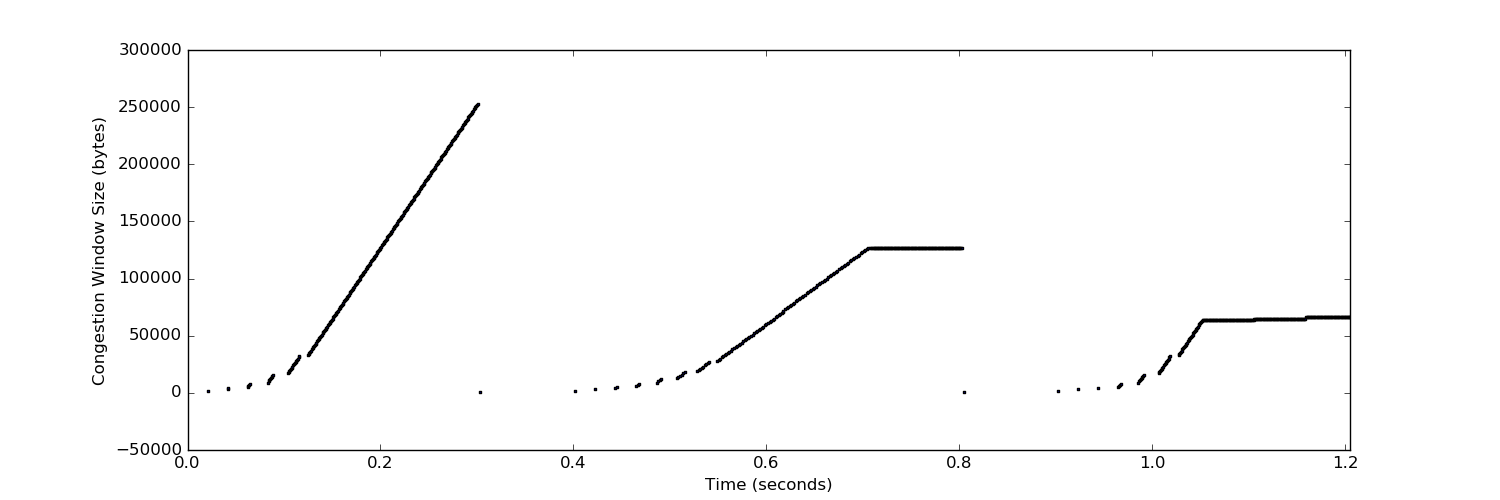
\includegraphics[width=\linewidth]{1f_window.png}
\end{figure}

\begin{figure}[H]
\caption{The graph of our one flow sequence plot.}
  \label{figure4}
    \centering
    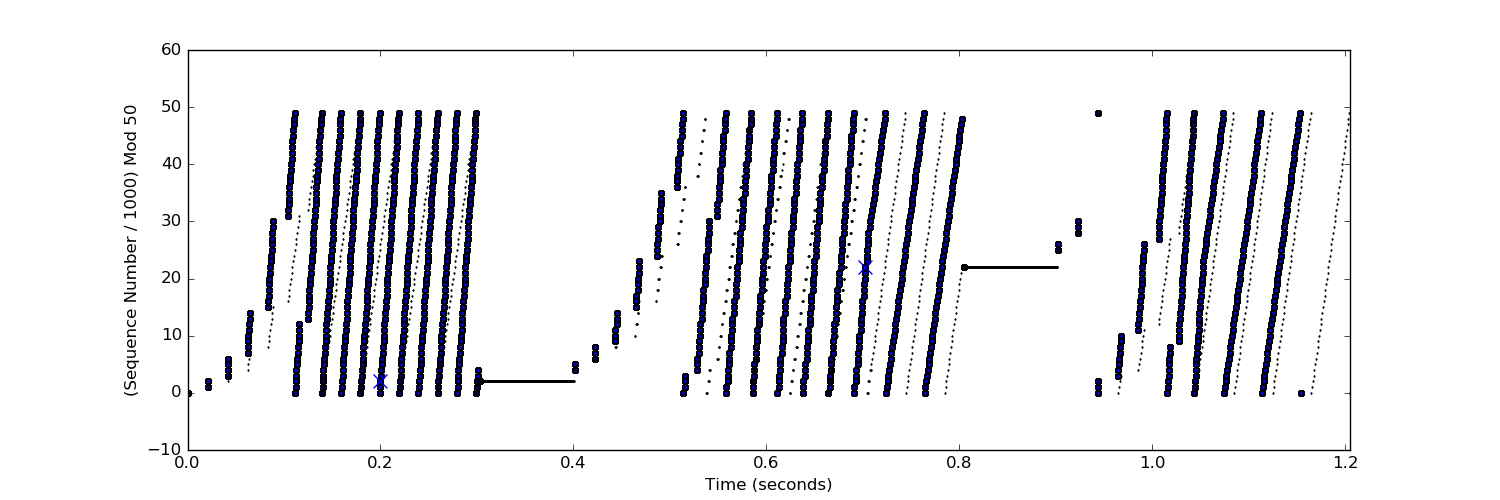
\includegraphics[width=\linewidth]{1f_seq.png}
\end{figure}

Figure 1 shows how the receive rate changes over time for a single flow. We can see that the receive rate goes up very quickly and levels off; this is expected behavior because the flow has access to the full bandwidth. In Figure 2 we see how the queue size is quickly filled during slow start because the threshold is much larger than the queue size. However after some loss, congestion control helps keep the queue size under its max of 100 packets. If the file that we transfered was larger than 1 MB, we would see the additive increase section at around 1.1 seconds continue without loss for a long time. Figure 3 supports Figure 2 by showing the typical saw tooth pattern that reflects TCP's attempt to find a congestion window size appropriate for the link. 

\subsection{Two Flow}

\begin{figure}[H]
\caption{The graph of our two flow receivers' rates over time.}
  \label{figure5}
    \centering
    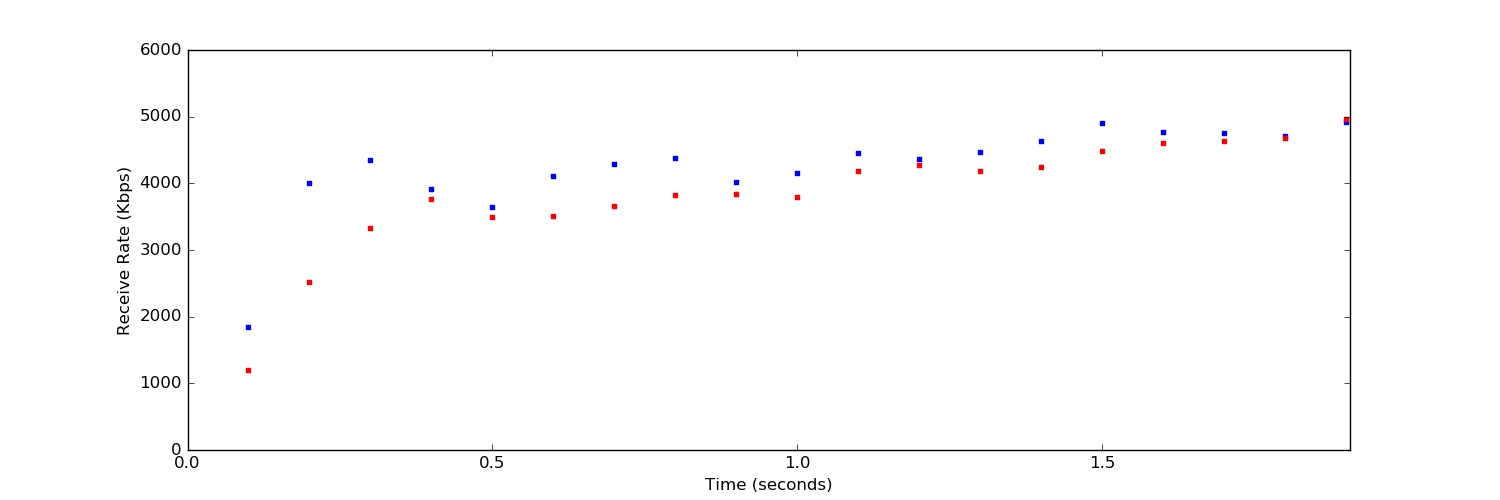
\includegraphics[width=\linewidth]{2f_rate.png}
\end{figure}

\begin{figure}[H]
\caption{The graph of our two flow queue size over time.}
  \label{figure6}
    \centering
    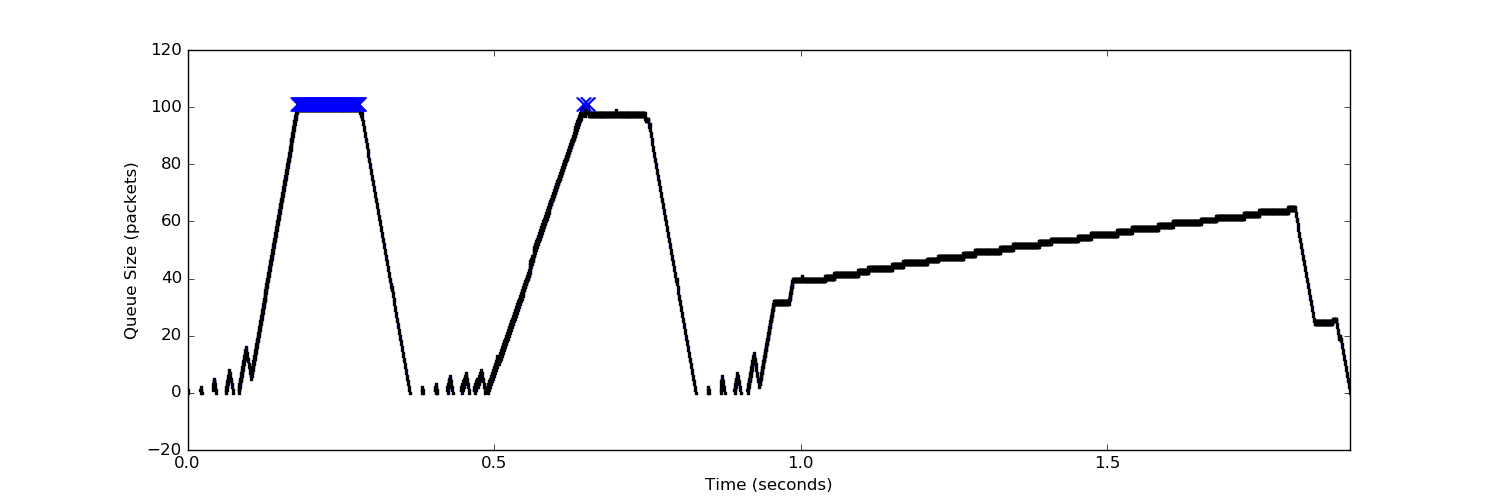
\includegraphics[width=\linewidth]{2f_queue.png}
\end{figure}

\begin{figure}[H]
\caption{The graph of our two flow congestion window size over time for flow A.}
  \label{figure7}
    \centering
    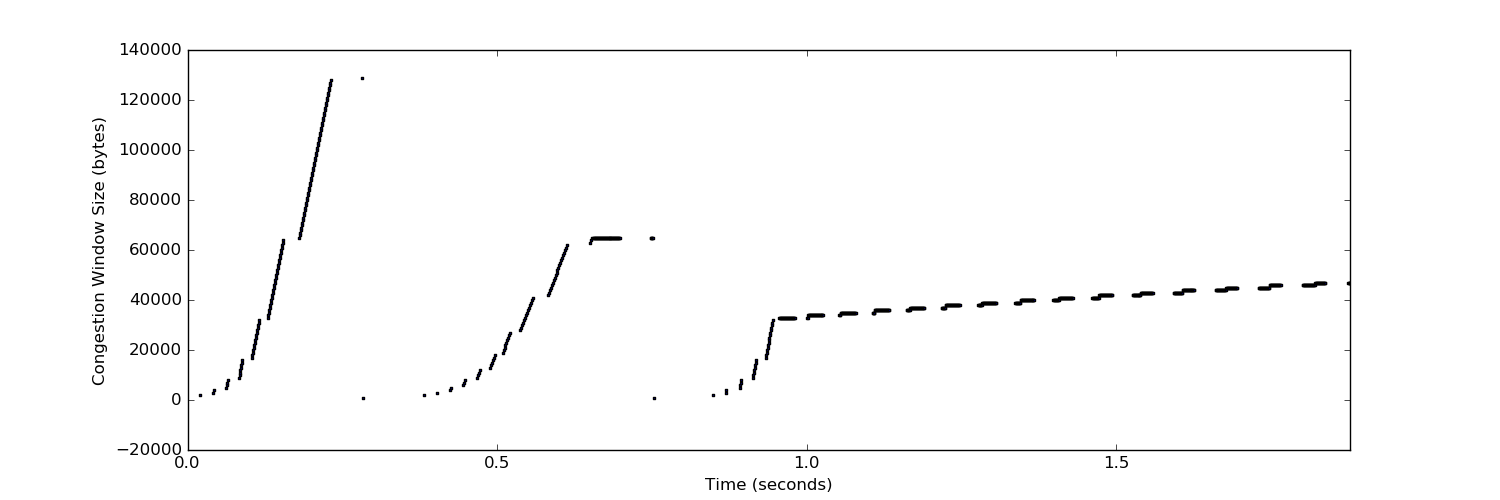
\includegraphics[width=\linewidth]{2f1_window.png}
\end{figure}

\begin{figure}[H]
\caption{The graph of our two flow congestion window size over time for flow B.}
  \label{figure8}
    \centering
    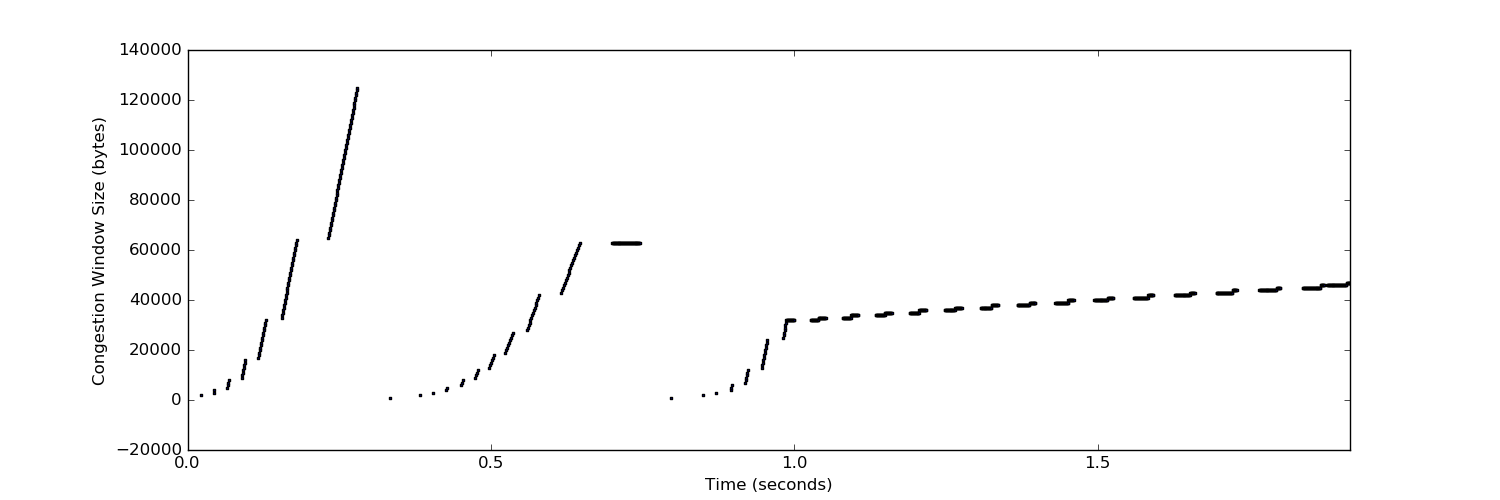
\includegraphics[width=\linewidth]{2f2_window.png}
\end{figure}

\begin{figure}[H]
\caption{The graph of our two flow sequence plot for flow A.}
  \label{figure9}
    \centering
    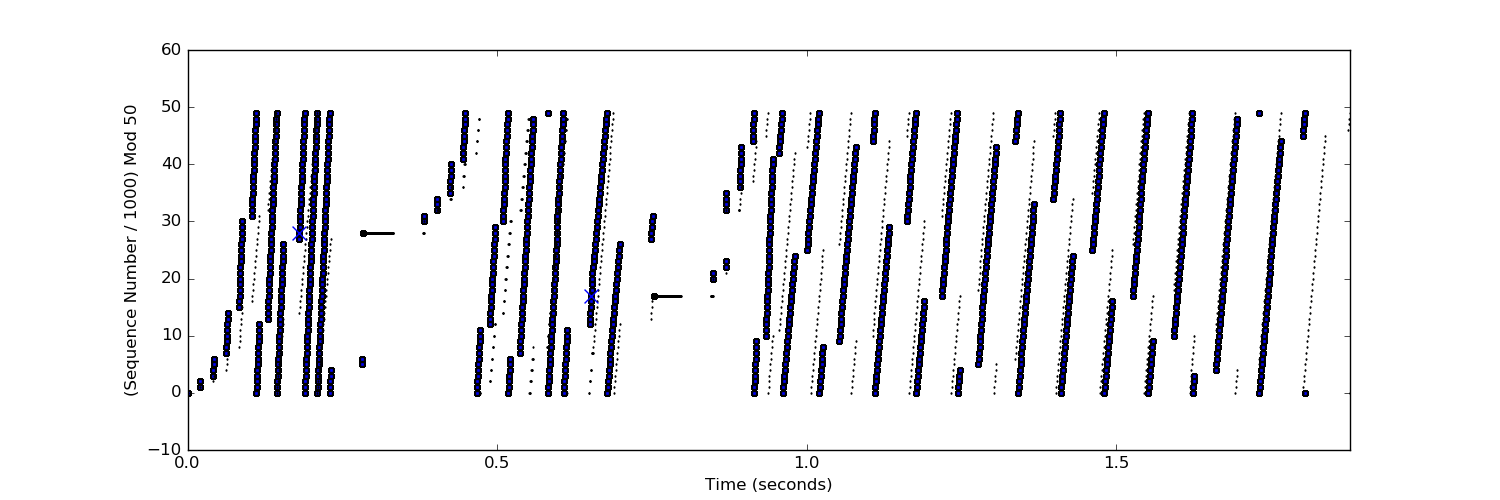
\includegraphics[width=\linewidth]{2f1_seq.png}
\end{figure}

\begin{figure}[H]
\caption{The graph of our two flow sequence plot for flow B.}
  \label{figure10}
    \centering
    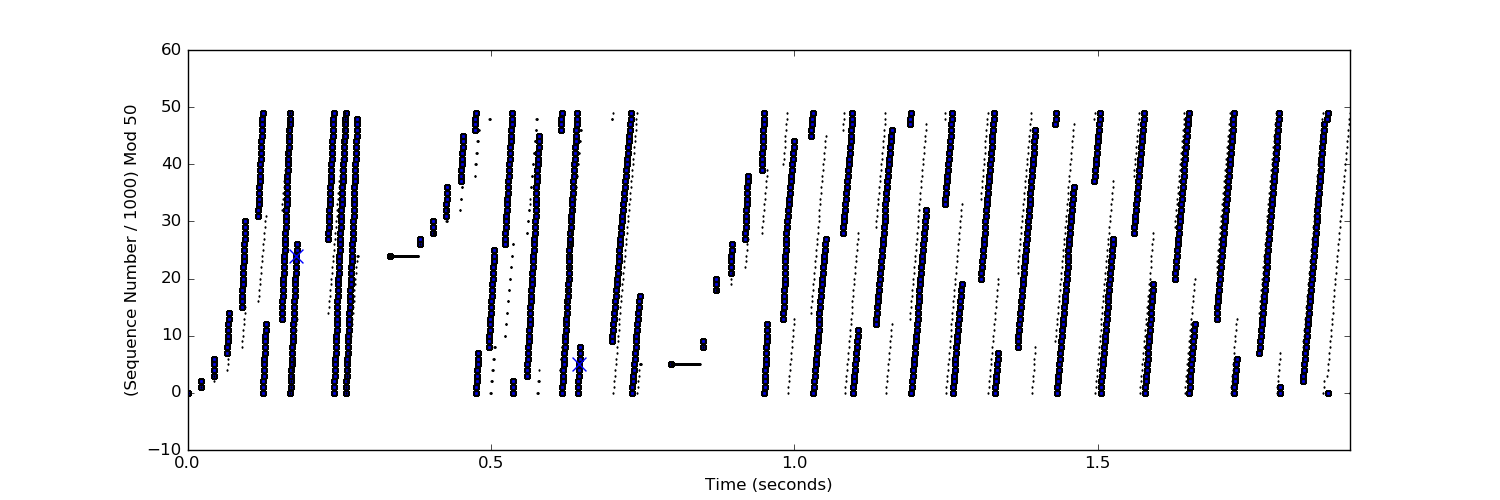
\includegraphics[width=\linewidth]{2f2_seq.png}
\end{figure}

Because the two flows in this experiment were identical, we would expect both data series in Figure 5 to look nearly identical. Figure 5 shows this behavior. We would also expect Figures 7 and 8 to look nearly identical because both flows experience loss at nearly the same time and adjust their windows to the same values. Figures 7 and 8 do look nearly identical as expected. Figure 6 also demonstrates expected behavior; this is clear particularly when you compare Figure 6 with Figure 2. On both graphs we see two peaks loss events occuring while TCP is still identifying a good window for the link. After the second peak both flows start additive increase before the queue is filled. However, in Figure 6 the slope of the increase in queue size during the additive increase period is steeper than the slope in Figure 2 because Figure 6 shows two flows, both doing additive increase. 

\subsection{Five Flow}

\begin{figure}[H]
\caption{The graph of our five flow receivers' rates over time.}
  \label{figure11}
    \centering
    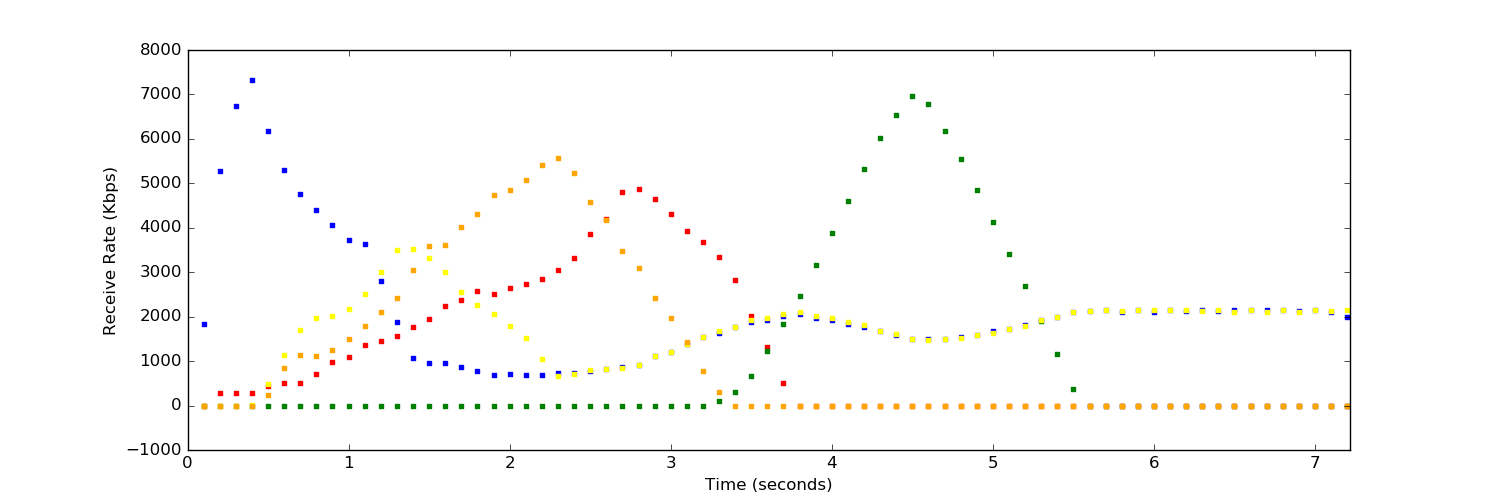
\includegraphics[width=\linewidth]{5f_rate.png}
\end{figure}

\begin{figure}[H]
\caption{The graph of our five flow queue size over time.}
  \label{figure12}
    \centering
    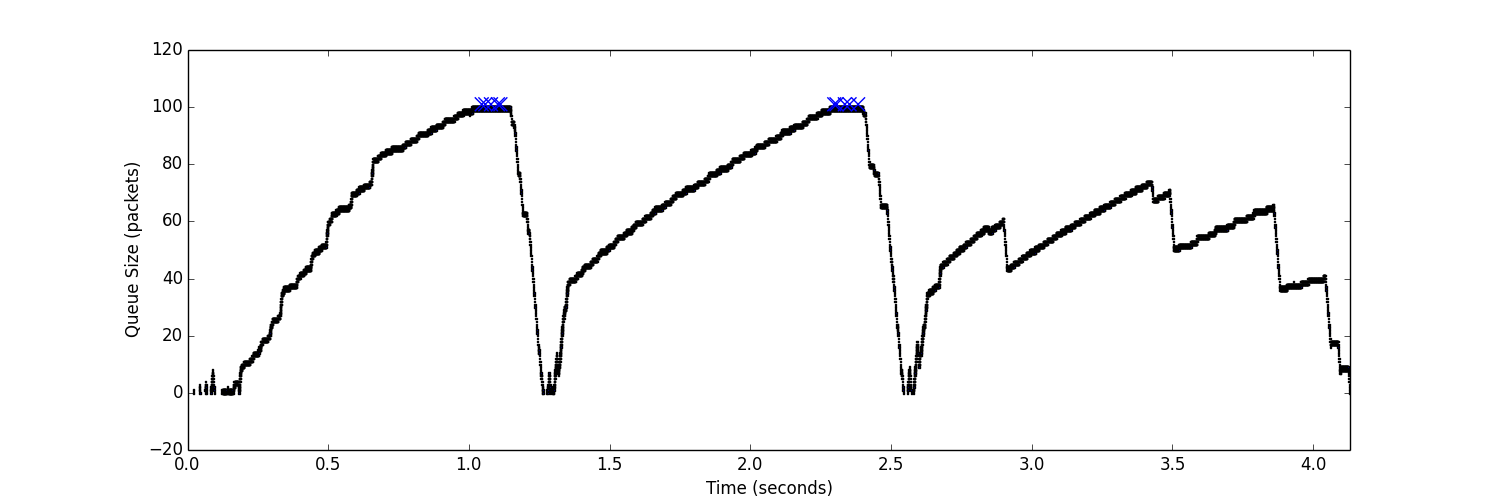
\includegraphics[width=\linewidth]{5f_queue.png}
\end{figure}

For five flow we decided a smaller threshold size of 16,000 bytes. We chose to do this because with such a small file there was not enough time for the TCP connections to balance their share of the link before flows started finishing their file transfer. Five flow also differed from one and two flow because each flow began transfering 0.1 seconds after the preceeding flow (i.e. 0.0, 0.1, 0.2, 0.3, 0.4).

In a correct implementation of TCP, the first flow to begin transferring will immedietely take advantage of all the bandwidth. As more connections begin sharing the link the receive rate of the initial flows should drop while the receive rate of the newer flows should increase until they are roughly the same. This means that they are equally sharing the bandwidth. As early flows finish transferring their files the remaining flows start to take advantage of the newly available bandwidth. Figure 11 is evidence of this behavior. 

\section{Advanced Experiments}


\subsection{Additive Increase - Additive Decrease (AIAD)}

\begin{figure}[H]
\caption{The graph of our one flow receiver's rate over time with AIAD.}
  \label{figure13}
    \centering
    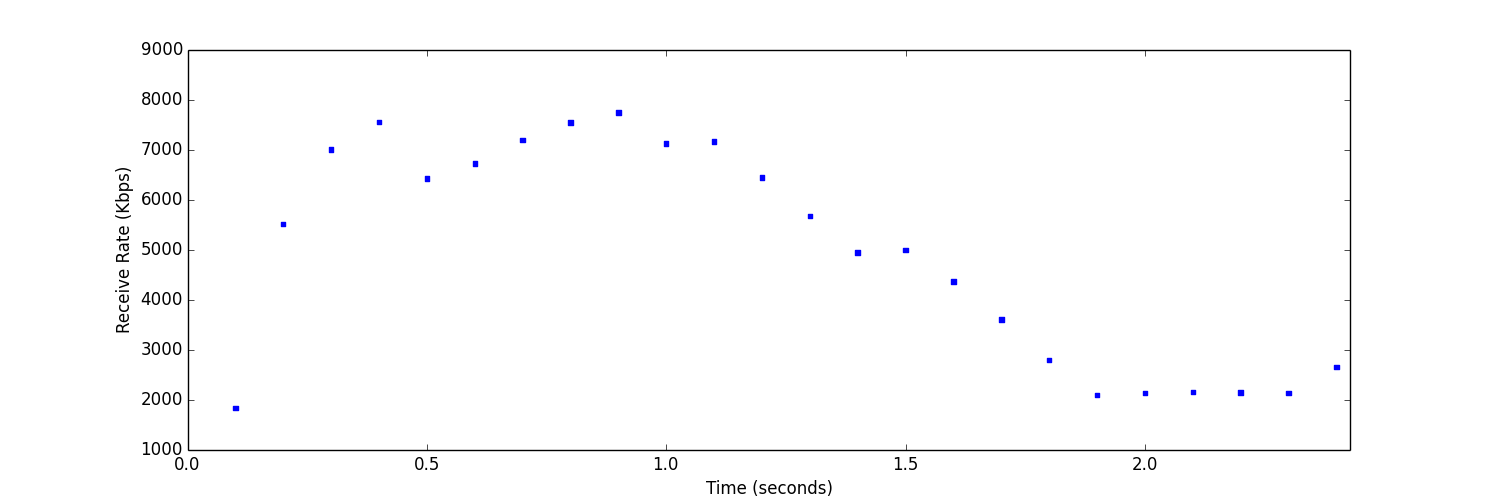
\includegraphics[width=\linewidth]{1f_rateAIAD.png}
\end{figure}

\begin{figure}[H]
\caption{The graph of our one flow congestion window size over time with AIAD.}
  \label{figure14}
    \centering
    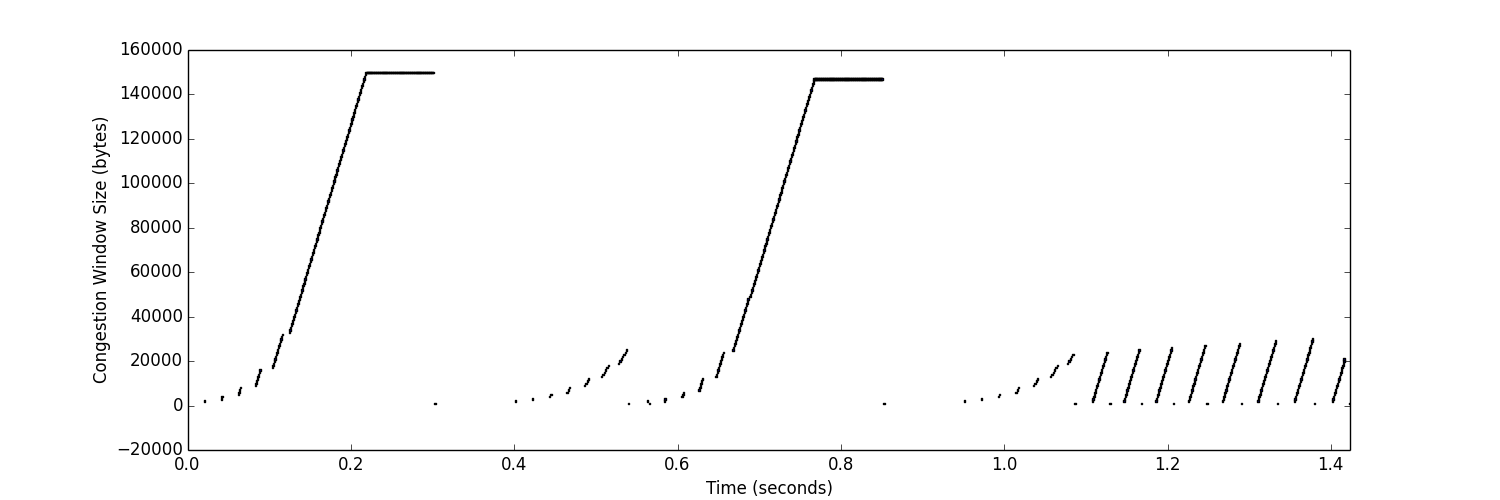
\includegraphics[width=\linewidth]{1f_windowAIAD.png}
\end{figure}

AIAD differs from standard TCP in one main way: instead of reducing the TCP threshold by half after a loss event, we reduce the threshold by 1000 bytes (1 packet). The performance of this method of congestion control could have decent results with a single flow on a single stable link with a threshold below the queue size; however, if any of those elements are not present, the threshold will take a while to shift below the queue size, which means that slow start will repeatedly overflow the queue.

In our experiment, we used one flow with a threshold that was much larger than the queue size, so our performance was much worse than if we had reduced the window by ½ after each loss event. By comparing Figure 1 and Figure 13, we can see that the file transfer took twice as long with AIAD. Figure 14 shows how loss events quickly manifested themselves and repeated. Because the file was only 1MB, the pattern of quick peaks and losses only happens twice, but with a larger file we would see this pattern continue.


\subsection{Additve Increase - 5/6 Multiplicative Decrease (AIMD)}

\begin{figure}[H]
\caption{The graph of our one flow receiver's rate over time with a 5/6 multiplicative decrease.}
  \label{figure15}
    \centering
    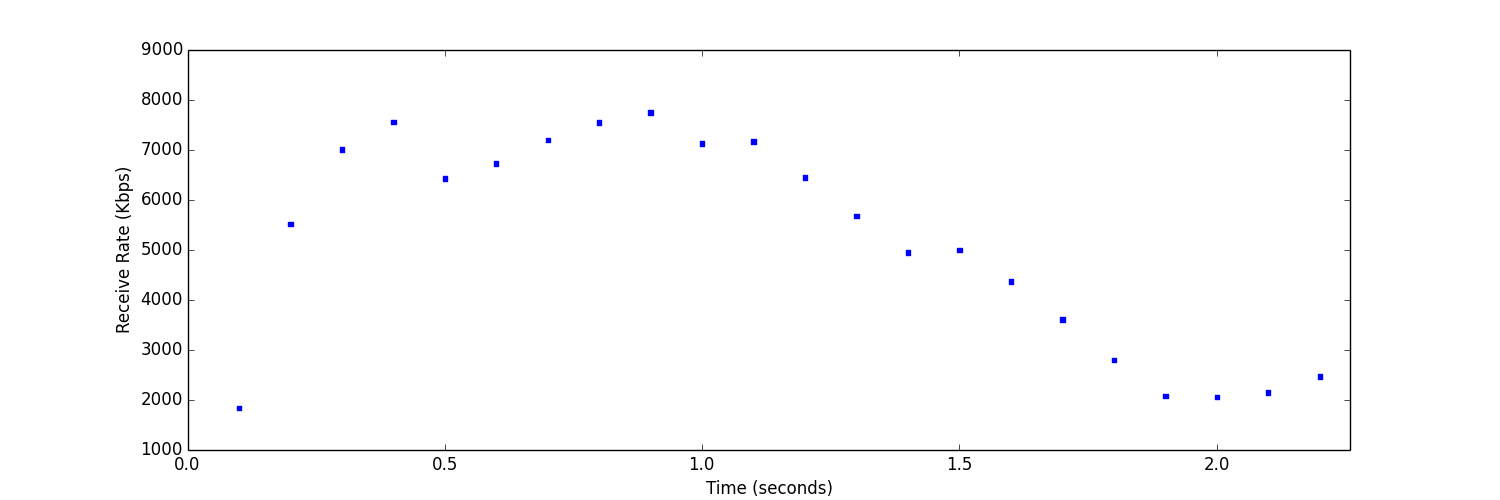
\includegraphics[width=\linewidth]{1f_rateAIMD.png}
\end{figure}

\begin{figure}[H]
\caption{The graph of our one flow congestion window size over time with a 5/6 multiplicative decrease.}
  \label{figure16}
    \centering
    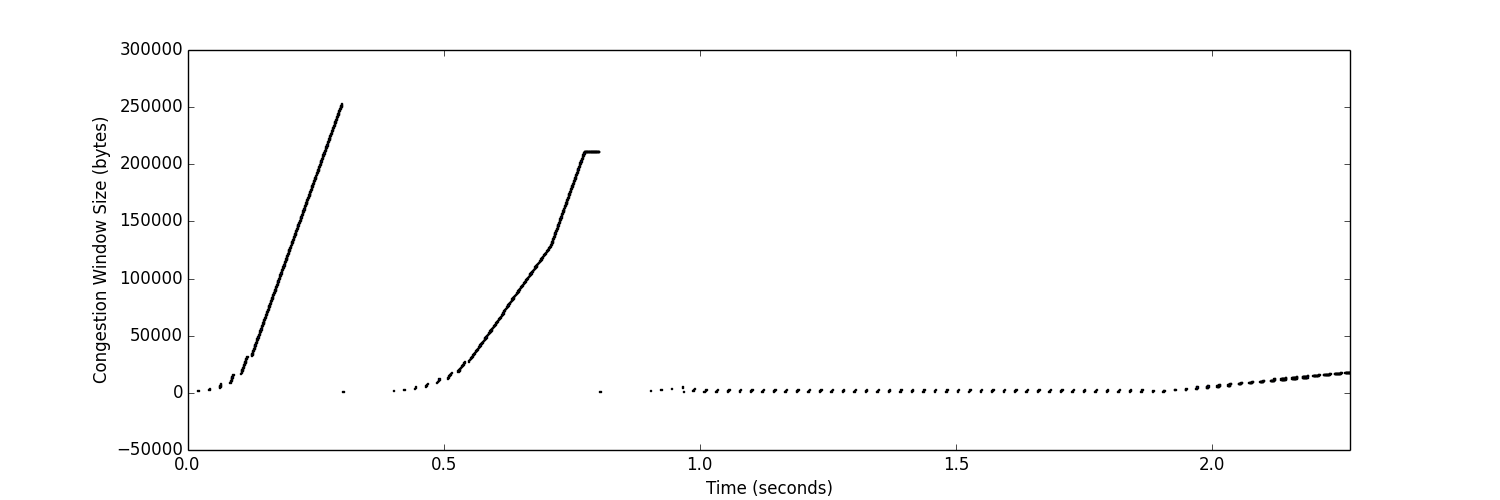
\includegraphics[width=\linewidth]{1f_windowAIMD.png}
\end{figure}

This implementation of TCP still uses multiplicative decrease, but instead of reducing the TCP threshold by half after a loss event, we reduce the threshold to ⅚ the size. Given enough time and a large enough file, we would still expect this method to produce reasonably stable performance, assuming the link is fairly stable. 

The performance of this version of AIMD was similar to that of AIAD. Throughput is much worse than if the window size was reduced by half because it takes longer for the threshold to decrease below the queue size. As long as the threshold is greater than the max queue size, slow start will max out the queue and cause loss. Using AIMD with a factor of ⅚ does bring the threshold down more quickly than AIAD, which can be seen by comparing Figure 14 to Figure 16 where the congestion window size decreases more quickly. Using this version of AIMD also give slightly better throughput, which is shown by a comparison of Figure 13 and Figure 15. Figure 15 shows AIMD transferring the file in about 2 seconds, while Figure 13 shows AIAD transferring the file in about 2.5 seconds.

\subsection{Competing AIMD}

\begin{figure}[H]
\caption{The graph of our two flow receivers' rates over time with competing AIMD.}
  \label{figure15}
    \centering
    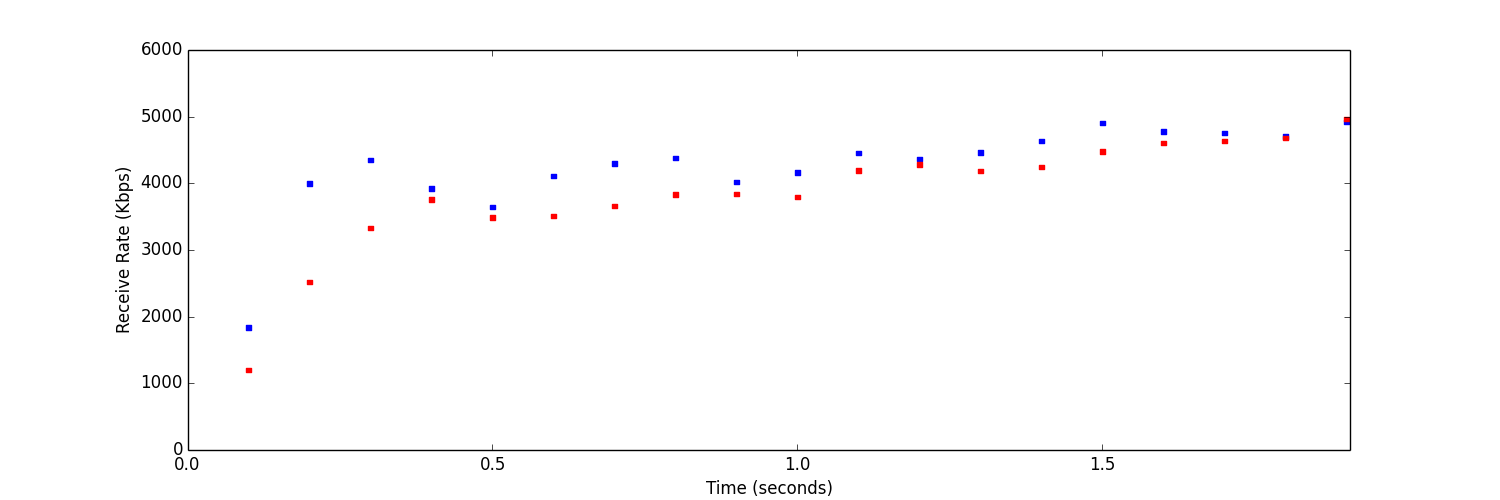
\includegraphics[width=\linewidth]{2f_rateAIMD.png}
\end{figure}

For this experiment we had two flows using AIMD sharing the link. However, the first flow (shown in blue) used a ½ multiplier to decrease its threshold size and the second flow (shown in red) used a ⅚ multiplier to decrease its threshold size.

As discussed in section 3.2, performance for any version of TCP will be strongly affected by how quickly the threshold can drop to a value below the maximum queue size. In this experiment the first loss event happens at around t = 1 second. However after decreasing their respective thresholds, the combined threshold value was still too large for the link’s queue to handle. After the second loss event at t = 2 seconds, the combined queue size is more reasonable for the link because the flow with a ½ constant decreased its threshold by a significant amount. The threshold for the flow with a ⅚ is much higher than that of the other flow, so its throughput is much higher.

We can see this in Figure 17 because the red data series, which corresponds to the flow with a ⅚ constant, is much higher after the second loss event at t = 2 seconds, whereas the blue series drops much lower because of its lower threshold. This is what we would expect for these competing versions of TCP.

\subsection{Competing Round Trip Time (RTT)}

\begin{figure}[H]
\caption{The graph of our two flow receivers' rates over time with competing RTT.}
  \label{figure16}
    \centering
    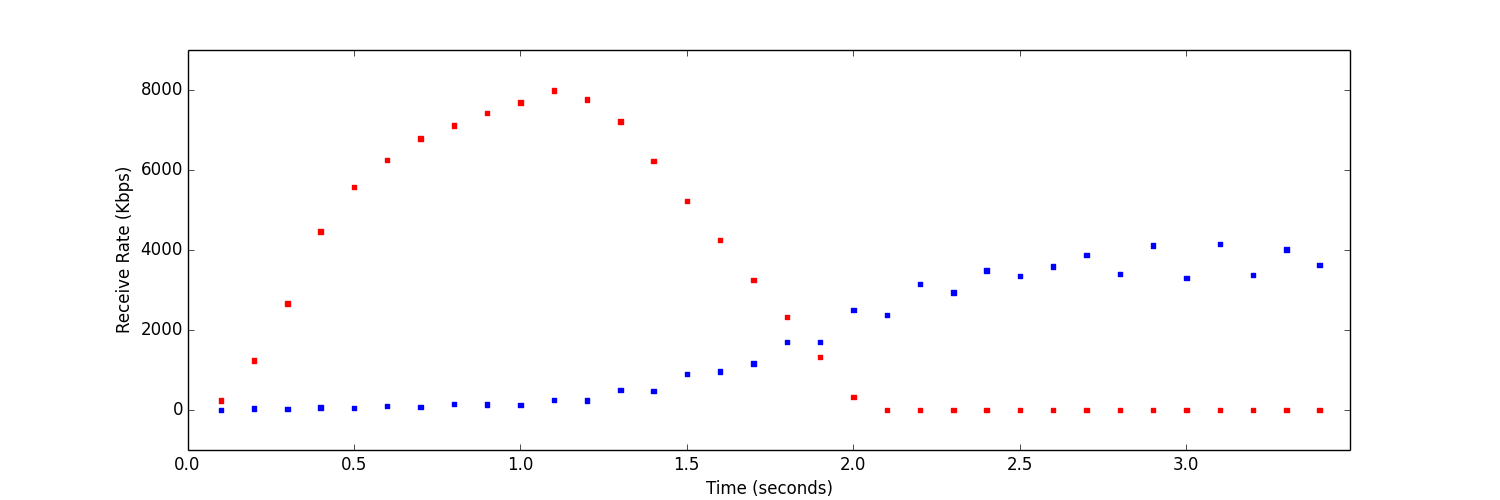
\includegraphics[width=\linewidth]{2f_rate_rtt.png}
\end{figure}

For this experiment we had two flows using identical AIMD. The difference was that the first flow (blue) had a propagation delay of 100 ms and the second flow (red) had a propagation delay of 10 ms. 

The expected behavior for this environment is that the faster link will get much higher throughput than that of the slower link. There are two main reasons for this. First, when the combined congestion windows are smaller than the max queue size, the flow with the slower link takes longer to receive ACKs for the packets that it transmits and therefore takes longer to increase its congestion window size. The second reason is that, when the combined congestion windows are larger than the max queue size, the packets for the faster link will arrive at the queue before the packets for the slow link. This means that when the packets from the fast link get to the queue, the queue is small, but when the packets from the slow link arrive the queue, the queue is too full to accept all of the packets.

Figure 18 shows that the first flow has a much larger portion of the available bandwidth until it finishes sending its 1 MB file. At this point the second flow begins to use up the newly available bandwidth, albeit slower than flow one because of the extra time it takes to receive ACKs thereby increasing its congestion window size.

\end{document}
